\documentclass[xcolor=dvipsnames,9pt,mathserif]{beamer}

\usetheme{Yendor}

\usepackage{amsmath,amsfonts,amssymb,eurosym,ulem}
\usepackage{graphicx,pgf,tikz,fancyvrb,listings}
\usepackage{alltt}
\usepackage[english]{babel}
\usepackage[utf8]{inputenc}
\usepackage{multirow}

\usetikzlibrary{mindmap}

\graphicspath{{images/}}

\definecolor{lightgray}{rgb}{.92,.92,.92}
\definecolor{darkgreen}{rgb}{0,.4,0}
\definecolor{darkblue}{rgb}{0,0,.5}

\boldmath

\def\N{\mathbb{N}}		%Les entiers naturels
\def\CP{\mathcal{CP}}		%horloges binaires parenthèsées
\def\oncp{\on^{\CP}}
\def\CB{\mathcal{CB}}		%horloges binaires
\def\CBC{\mathcal{CB_{()}}}	%horloges binaires périodiques
\def\CN{\mathcal{CN}}		%horloges entières
\def\CNC{\mathcal{CN_{()}}}	%horloges entières périodiques/cycliques
\def\CR{\mathcal{CR}}
\def\apn{\alpha_{p\to n}}
\def\on{\,\mathtt{on}\,}
\def\dr{\,\mathtt{dr}\,}
\def\fby{\,\mathtt{fby}\,}
\def\when{\,\mathtt{when}\,}
\def\pre{\,\mathtt{pre}\,}
\def\merge{\,\mathtt{merge}\,}
\def\not{\,\mathtt{not}\,}
\def\pos{\,\mathtt{pos}\,}
\def\index{\,\mathtt{index}\,}
\def\by{\,\mathtt{by}\,}
\def\half{\,\mathtt{half}\,}

% les opérateurs sémantiqués
\def\is{i^\sharp\,}
\def\ops{op^\sharp}
\def\fbys{\mathtt{fby}^\sharp}
\def\ffbys{\mathtt{f\_fby}^\sharp}
\def\lfbys{\mathtt{l\_fby}^\sharp}
\def\whens{\mathtt{when}^\sharp}
\def\bwhens{\mathtt{b\_when}^\sharp}
\def\swhens{\mathtt{s\_when}^\sharp}
\def\merges{\mathtt{merge^\sharp}}
\def\bys{\mathtt{by^\sharp}}
\def\sbys{\mathtt{s\_by^\sharp}}
\def\bbys{\mathtt{b\_by^\sharp}}

\def\ENV#1#2#3{\left\langle #1, #2\right\rangle \left(#3\right)}
\def\Abs{\textrm{Abs}}
\def\Buffer{\textrm{Buffer}}
\def\Delay{\textrm{Delay}}

\newenvironment{chrono}{\begin{math}\begin{array}{r|llllllllllll}}{\end{array}\end{math}}
\def\li{\\ \hline}
\def\t{\texttt{\color{darkblue}\textit{t}}}
\def\f{\texttt{\color{darkblue}\textit{f}}}

\newcommand{\bb}[1]{\textcolor{blue}{#1}}
\newcommand{\cc}[1]{\textcolor{DarkOrchid}{#1}}
\newcommand{\ccc}[1]{\textcolor{BurntOrange}{#1}}

\newcommand{\pdftex}[2][1]{\scalebox{#1}{\input{#2.pdf_t}}}
\renewcommand{\emph}[1]{\alert{#1}}
\newcommand{\code}[1]{\texttt{\color{darkgreen}#1}}

%% General shortcuts

\def\le{\leqslant}
\def\ge{\geqslant}
\def\from{\mathrel{\leftarrow}}
\def\imply{\mathrel{\Longrightarrow}}
\def\eps{\varepsilon}
\def\Alpha{\mathrm{A}}
\def\Beta{\mathrm{B}}
\def\Mu{\mathrm{M}}
\def\Bbb{\mathbb{B}}
\def\Nbb{\mathbb{N}}
\def\Zbb{\mathbb{Z}}
\def\Qbb{\mathbb{Q}}
\def\Rbb{\mathbb{R}}
\def\Mcal{\mathcal{M}}
\def\Ocal{\mathcal{O}}

\lstdefinelanguage{ccvm}{%
  %% Definition du langage
  %% List of keywords
  keywords={[1]for,do,while,if,else,break,continue,return,%
    returns,node,obc,let,tel,method,mem},
  keywords={[2]stream,const,volatile,static,signed,unsigned,%
    void,char,short,long,int,float,double,boolean,%
    size_t,rec_t,pixel_t,event_stamp_t,stamped_rec_t,item_t,sint16},
  keywords={[3]omp,pragma,parallel,num_threads,single,task,taskwait,async,%
    private,shared,firstprivate,lastprivate,nowait,schedule,%
    record,view,process,run,commit,update,receive,receive_range,%
    push,pop,%
    release,stall,set_number_registered,%
    spawn,sync,cilk,%
    spawn_async_process,sync_all_tasks,ask_for_work,%
    inquire_event,inquire_release,is_live,init,register,allocate},
  keywords={[4]input,output,team,history,%
    assert,rt_ns,atomic_cas,%
    load_load_fence,load_store_fence,store_load_fence,store_store_fence},
  emph={main,reset,step,astep,pipe,get,fast,slow,%
    producer,consumer,master,selector,compute,hscan,sync_av,%
    filter,pip_selector,pip,reduce,accumulate},
  %% List of abbreviations
  % literate={<=}{{$\leq$}}1 {>=}{{$\geq$}}1 {!=}{{$\neq$}}1 {*}{{$\times$}}1,
  %% List of strings
  literate={<<}{{\textbf{\color{red}<\hskip-1pt<}}}1 {>>}{{\textbf{\color{red}>\hskip-1pt>}}}1%
  {\#pragma}{{\textbf{\color{darkgreen}\#pragma }}}1,
  string=[b]",
  %% List of comment strings
  comment=[l]//,
  morecomment=[s]{/*}{*/},
  %% Special character for LaTeX
  mathescape=true,
  %% Definition du style
  flexiblecolumns=true,
  tabsize=2,
  %% numerotage des lignes
  %firstnumber=1,
  %stepnumber=1,
  %numbers=left,
  % numbersep=-6mm,
  %% titre
  captionpos=b,
  % abovecaptionskip=3mm,
  % belowcaptionskip=3mm,
  %% La boite englobante
  % frame=,
  aboveskip=1mm,
  belowskip=0mm,
  framesep=0mm,
  %% Les styles
  basicstyle=\ttfamily\footnotesize,
  keywordstyle={[1]\color{darkblue}},
  keywordstyle={[2]\color{darkgreen}},
  keywordstyle={[3]\color{orange}},
  keywordstyle={[4]\color{red}},
  %keywordstyle=\fontseries{bx}\fontfamily{cmss}\fontshape{n}\selectfont,
  % numberstyle=\footnotesize,
  % basicstyle=,
  % keywordstyle=\sbf,
  % numberstyle=,
  emphstyle=\color{blue},
  %identifierstyle=\color{blue},
  commentstyle=\color{darkgray}\scriptsize,
  stringstyle=\color{green},
}

\lstset{language=ccvm,%backgroundcolor=\color{lightgray},%
  frame=single,framerule=0pt}

\title[]{Semantics, languages and algorithms for multicore programming}

\author{\textbf{Albert Cohen}}

\institute{INRIA and École Normale Supérieure\\
  \url{http://www.di.ens.fr/ParkasTeam.html}}

\date{Third course, January 5, 2012}

\begin{document}

\begin{frame}
  \titlepage
  \vfill
%  
\includegraphics[height=1.2cm]{logo_nn.pdf} \hfill \includegraphics[height=1.2cm]{gnu.png} \hfill \includegraphics[height=.65cm]{inria.pdf}
  \bigskip
  \hfill \includegraphics[height=.8cm]{logoinria.jpg} \hfill
\end{frame}

% \begin{frame}
% \begin{center}
%   \Large\bf {PARKAS} Team\\
%   {\color{blue}S}ynchronous {\color{blue}Ka}hn {\color{blue}Par}allelism
% \end{center}

% \bigskip
% New research group established in September 2010

% \bigskip
% 4 permanent researchers
% \begin{center}
% \begin{tabular}{cccc}
%     Marc Pouzet & Jean Vuillemin & Albert Cohen & Louis Mandel \\
% %
%     \includegraphics[scale=.35]{images/pouzet.pdf} 
% &
%     \includegraphics[scale=.35]{images/vuillemin.pdf} 
% &
%     \includegraphics[scale=.35]{images/cohen.pdf} 
% &
%     \includegraphics[scale=.35]{images/mandel.pdf} 
% \\
% \end{tabular}
% \end{center}

% \bigskip
% 2 post-docs, 11 PhD students, 1 engineer, 1 master student

% \smallskip
% \centerline{\url{http://www.di.ens.fr/ParkasTeam.html}}
% \end{frame}

\section{Multicore Processors: Why Should We Bother?}

\begin{frame}[t]
  \frametitle{Stored Program, von Neumann Architecture}
  \begin{center}
    \includegraphics[width=3cm]{von_neumann_architecture.png}
  \end{center}

  \begin{block}{}
    \begin{itemize}
    \item IAS Architecture, John von Neumann
    \item SSEM ``Baby'', 1948: Tom Kilburn, Victoria U. of Manchester

      First implementation of the \emph{stored program} concept in a
      real machine
    \item EDVAC, 1949: John Eckert, J.\ Presper Mauchly and John von Neumann
    \end{itemize}
  \end{block}
\end{frame}

\begin{frame}{Moore's Law on Silicon Semiconductors}
  \centerline{\includegraphics[width=10cm]{Moores_Law.jpg}}
\end{frame}

\begin{frame}{Evolutions of the von Neumann Architecture}
  \begin{block}{What Can We Do With All These Transistors?}
    \begin{itemize}
    \item 60+ years of evolution
      \begin{itemize}
      \item Registers
      \item Cache (local memory, memory hierarchy)
      \item Instruction pipeline
      \item Branch predictor, prefetch, speculative execution
      \item Superscalar execution, out-of-order execution

        \medskip
      \item<2-> \slshape Multi-thread processor
      \item<2-> \slshape Multi-processors, multi-core, many-core
      \item<2-> \slshape Specialization (hardware accelerators)
      \end{itemize}
    \item<3> Is it the end of the road for the von Neumann architecture?
    \end{itemize}
  \end{block}
\end{frame}

\begin{frame}{Algorithms, Programming Languages, and Multicore Processors?}
  \begin{enumerate}
  \item Discrete Mathematics, Computing Science,

    Computer Science, Computer Engineering?

    \vskip-1cm
    \hfill\includegraphics[width=3cm]{dijkstra.jpg}
    
    \begin{center}
      \emph{``Computer science is no more about computers \\
        than astronomy is about telescopes''}

      \medskip
      Edsger Dijkstra (1930--2002), Turing Award 1972
    \end{center}
  \item Let's talk about \emph{telescopes and astronomy}: telescope
    builders and astromomers interact a lot, there must be a reason
  \end{enumerate}
\end{frame}

\section{Telescopes}

\begin{frame}{More Moore}
  \centerline{\includegraphics[width=8cm]{Moores_Law_and_more.jpg}}

  {\footnotesize From Olukotun, Sutter and Hammond}
\end{frame}

\begin{frame}{Memory Wall}
  \begin{center}
    \begin{tabular}{|l|l|l|}
      \hline
      Memory & Latency & Peak Bandwidth (dual-channel) \\
      \hline
      DDR2-400 SDRAM & $15$ ns & $6.4$ GB/s \\
      DDR2-533 SDRAM & $11.3$ ns & $8.5$ GB/s \\
      DDR2-667 SDRAM & $12$ ns & $10.7$ GB/s \\
      DDR2-800 SDRAM & $10$ ns & $12.8$ GB/s \\
      DDR2-1066 SDRAM & $11.3$ ns & $17.6$ GB/s \\
      \hline
    \end{tabular}
  \end{center}

  \bigskip
  Compared to a 4-core 3GHz Core 2 processor:

  \qquad Latency: $0.33$ ns

  \qquad Bandwidth: $4\textrm{ threads}\times 2\textrm{ L/S units}\times 16\textrm{ bytes}\times 3=384$ GB/s
\end{frame}

\begin{frame}[t]{Multicore Processors}
  \begin{center}
    \bfseries
    \begin{minipage}[b]{4.3cm}
      \centering
      \includegraphics[width=\textwidth]{parallelism.jpg}

      Parallelization
    \end{minipage}
    \hfill
    \begin{minipage}[b]{3.5cm}
      \centering
      \includegraphics[width=\textwidth]{power.jpg}

      Power management
    \end{minipage}
    \hfill
    \begin{minipage}[b]{3.9cm}
      \centering
      \includegraphics[width=\textwidth]{cheese.jpg}

      Specialization
    \end{minipage}
  \end{center}

  \begin{block}{Not (always) the fault of the telescope builder}
    \begin{center}
      \only<1>{%
        Recurrent costs \\
        $\downarrow$ \\
        Parallelism and specialization
        (for computational density and energy-efficiency) \\
        $\downarrow$ \\
        \emph{\textbf{Heterogeneity}}
        (on the chip, in the ecosystem)
      }%
      \only<2>{%
        \begin{tabular}{rcl}
          Non-recurring costs \hskip-1cm & &
          \hskip-1cm Variety and size of the applications \\
          $\searrow$ & & $\swarrow$ \\
          & \emph{\textbf{Programmability, portability}} &
        \end{tabular}
      }%
      \only<3>{%
        Unfortunately, more and more programmers are forced to think
        about the target architecture's features and constraints, and
        manually optimizing their codes}
    \end{center}
  \end{block}
\end{frame}

\begin{frame}{Example: Discrete Fourier Transform on 2
    Dual-Core Processors}
  \begin{center}
    \includegraphics[width=12cm]{dft1.png}
  \end{center}
\end{frame}

\begin{frame}{Example: Discrete Fourier Transform on 2
    Dual-Core Processors}
  \begin{center}
    \includegraphics[width=12cm]{dft2.png}
  \end{center}
\end{frame}

\begin{frame}[c]{Impact of Multicore Processors}

  {\large \textbf{The memory and power walls are here to stay}}

  \bigskip
  {\large \textbf{No performance gains outside parallelism or specialization}}

  \bigskip
  {\large \textbf{The end of ``weak scaling''}}
\end{frame}

\section{Astronomy}

\begin{frame}[c]{About Astronomy (Algorithms, Programming Languages)}

  {\large \textbf{What are the essential semantic requirements for source programs?}}

  \bigskip
  {\large \textbf{Which programmers should really care?}}

  \bigskip
  {\large \textbf{What role for the software stack (compilers, runtime libraries)?}}
\end{frame}

\begin{frame}{Scott Topology}
  \hfill\includegraphics[width=3cm]{scott.jpg}
  
  \begin{block}{Domain Theory}
    Dana Scott (1932--), Turing Award 1976

    \medskip    
    Denotational semantics of a system of recursive equations, defined
    as the least fixpoint of a system of equations over
    \emph{continuous} functions
  \end{block}
    
  \vfill
  \begin{itemize}
  \item[$\to$] General recursion
  \end{itemize}
\end{frame}  

\begin{frame}{Kahn Process Networks}
  \hfill\includegraphics[width=4cm]{kahn.jpg}
  
  \begin{block}{Kahn networks, 1974}
    Gilles Kahn (1946--2006)
    
    \medskip
    Denotationally: least fixpoint of a system of equations
    over \emph{continuous} functions on infinite \emph{streams}

    Languages: Lucid, SISAL, a lazy functional language is a special case
    
    \medskip
    Operationally: communicating processes over infinite
    FIFOs with blocking reads

    Many programming and modeling APIs

    \medskip
    See \textit{2.23.1. Synchronous Systems}
  \end{block}
    
  \vfill
  \begin{itemize}
  \item[$\to$] \emph{Deterministic} by construction
  \item[$\to$] General recursion and \emph{parallel composition}
  \end{itemize}
\end{frame}  

\begin{frame}{Lessons for Parallel Programmers}

  {\large \textbf{The need for parallelism in the machine code does
      not require the normal programmers to surrender decades of
      progress in the principles of programming languages and tools!}}

  \bigskip
  {\large \textbf{Runtime libraries and compiler writers have a lot of
      work and responsibilities...}}
  
  \bigskip
  \bigskip
  $\to$ We will now focus on runtime libraries and low-level programming models
  
  \medskip
  More about deterministic parallel programming and compilers on January 19
  
  More general ``well-behaved'' parallel programs and concurrent data
  structures by Luc Maranget.
\end{frame}

\section{1001 Threads}

\begin{frame}{Concurrency vs.\ Parallelism}
  \begin{block}{Fundamental Concepts}
    \emph{Parallelism} refers to the \emph{simultaneous} or
    \emph{overlapping} execution of concurrent operations

    \begin{itemize}
    \item Data parallelism
    \item Task parallelism
    \end{itemize}
  
    \emph{Locality}: at least as important for performance as the
    computation itself
  \end{block}
  
  \begin{block}{Hardware Point of View}
    \begin{itemize}
    \item Hardware Multi-Threading: interleaved or simultaneous, for
      latency hiding
    \item Flynn taxonomy: SIMD (vector), MISD (pipelining), MIMD
    \item NVidia's SIMT (CUDA)
    \item Levels of parallelism
    \item Grain of parallelism
    \end{itemize}
  \end{block}
  
  \begin{block}{Programming Style}
    \begin{itemize}
    \item SPMD (MPI), offloading (CUDA, OpenCL)
    \item Distributed/actors (Erlang)
    \item Skeletons (MapReduce)
    \end{itemize}
  \end{block}
\end{frame}

\begin{frame}
  \frametitle{Multi-Threaded Architectures}

  \begin{block}{Simultaneous Multi-Threaded (SMT)}
    \begin{itemize}
    \item A.k.a.\ hyper-threaded (Intel)
    \end{itemize}

    \centerline{\pdftex[.55]{threads_smt}}
  \end{block}
\end{frame}

\begin{frame}
  \frametitle{Cache-Coherent Multiprocessor Architectures}

  \begin{block}{Chip Multi-Processor (CMP)}
    \begin{itemize}
    \item A.k.a.\ multicore (Intel)
    \item Multiple cores interconnected one or more buses
    \item Snoopy caches: e.g., MESI protocol
    \end{itemize}

    \centerline{\pdftex[.55]{threads_cmp}}
  \end{block}
\end{frame}

\begin{frame}
  \frametitle{Cache-Coherent Multiprocessor Architectures}

  \begin{block}{Symmetric Multi-Processor (SMP)}
    \begin{itemize}
    \item Multiple chips interconnected one or more buses
    \item Snoopy caches
    \end{itemize}

    \centerline{\pdftex[.55]{threads_smp}}
  \end{block}
\end{frame}

\begin{frame}
  \frametitle{Cache-Coherent Multiprocessor Architectures}

  \begin{block}{Non-Uniform Memory Architecture (NUMA)}
    \begin{itemize}
    \item Multiple chips interconnected by a network
    \item Directory-based cache protocol
    \end{itemize}

    \centerline{\pdftex[.55]{threads_numa}}
  \end{block}
\end{frame}

\begin{frame}[c]{Logical Threads vs. Hardware Threads}
  \begin{block}{Logical Thread Abstraction}
    Multiple \emph{concurrent} execution contexts of the same program,
    cooperating over a single memory space, called \emph{shared
      address space} (i.e., shared data, consistent memory addresses
    across all threads)
  \end{block}

  Among the different forms of logical thread abstrations,
  \emph{user-level} threads do not need a processor/kernel
  context-switch to be scheduled
    
  \begin{block}{Mapping Logical to Hardware Threads}
    The hardware threads are generally exposed directly as operating
    system kernel threads (POSIX threads); these can serve as
    \emph{worker threads} on which user-level threads can be mapped

    Mapping strategies: one-to-one, many-to-one, \emph{many-to-many}
  \end{block}
\end{frame}

\begin{frame}{Logical Threads vs. Hardware Threads}
  \begin{block}{Thread ``Weight''}
    \begin{enumerate}
    \item Lightest: run-to-completion coroutines

      $\to$ indirect function call
    \item Very light: coroutines, fibers, protothreads,
      cooperative user-level threads

      $\to$ garbage collector, cactus stacks with generalized activation records
    \item Light: user-level threads

      $\to$ preemption support, register checkpointing
    \item Heavy: kernel threads (POSIX threads)

      $\to$ context switch
    \item Heavier: kernel processes

      $\to$ heavier context switch with page table operations (TLB flush)
    \end{enumerate}
  \end{block}
\end{frame}

\section{Mapping Logical Threads to Hardware Threads}

\begin{frame}[c]{Task Pool}
  General approach to schedule user-level threads

  \begin{itemize}
  \item Single task queue
  \item Split task queue for scalability and dynamic load balancing
  \end{itemize}

  \bigskip
  More than one pool may be needed to separate ready threads
  from waiting/blocked threads
\end{frame}

\begin{frame}{Task Pool: Single Task Queue}
  Simple and effective for small number of threads

  \bigskip
  Caveats:
  \begin{itemize}
  \item The single shared queue becomes the point of contention
  \item The time spent to access the queue may be
    significant as compared to the computation itself
  \item Limits the scalability of the parallel application
  \item Locality is missing all together
  \end{itemize}
\end{frame}

\begin{frame}[c]{Task Pool: Split Task Queue}
  \begin{block}{Work Sharing}
    Threads with more work push work to threads with less work
    A centralized scheduler balances the work between the
    threads
  \end{block}

  \begin{block}{Work Stealing}
    A thread that runs out of work tries to steal work from some
    other thread
  \end{block}
\end{frame}

\begin{frame}{The Cilk Project}
  \begin{itemize}
  \item Language for dynamic multithreaded applications
  \item C dialect
  \item Developed since 1994 at MIT in the group of Charles Leiserson

    \hfill\includegraphics[width=3cm]{leiserson}
    
    \url{http://supertech.csail.mit.edu/cilk}

    Now part of Intel Parallel Studio (and TBB, ArBB)
  \end{itemize}
\end{frame}

\begin{frame}[fragile]{Fibonacci in Cilk}
  \begin{itemize}
  \item Tasks are (nested) coroutines
  \item Two keywords:
    \begin{itemize}
    \item \texttt{spawn \textit{function}()} to indicate that the
      function call \emph{may} be executed as a coroutine
    \item \texttt{sync} to implement a \emph{synchronization barrier},
      waiting for \emph{all child tasks of the current task}
    \end{itemize}
  \end{itemize}

  \bigskip
  \begin{lstlisting}
  cilk int fib (int n) {
    if (n < 2)
      return n;
    else {
      int x, y;
      x = spawn fib (n-1);
      y = spawn fib (n-2);
      sync;
      return (x+y);
    }
  }
  \end{lstlisting}
\end{frame}

\begin{frame}[fragile]{Fibonacci in Cilk: Generated Code}
  \begin{minipage}{4cm}
    \begin{lstlisting}
  cilk int fib (int n) {
    if (n < 2)
      return n;
    else {
      int x, y;
      x = spawn fib (n-1);
      y = spawn fib (n-2);
      sync;
      return (x+y);
    }
  }
    \end{lstlisting}
  \end{minipage}
  \hfill
  \begin{minipage}{7cm}
    \includegraphics[width=7cm]{fib_cilk_generated}

    {\footnotesize From Frigo et al.\ 1998}
  \end{minipage}

  \medskip
  Optimizations: tail-call, memory management, throttling...
\end{frame}

\begin{frame}{Cilk Properties}
  Cilk programs are canonically sequentialized with the elision of the
  special keywords
  
  $\to$ Depth-first execution of the task tree by a single-thread

  \medskip
  \centerline{\includegraphics[width=8cm]{cilk_dag}}

  \bigskip
  $\to$ As a corollary, all inputs to a task are available at the
  task creation point
  
  $\to$ A property called strictness (some relation to
  strictness in functional languages)
\end{frame}
  
\begin{frame}{Cilk Properties}
  \begin{itemize}
  \item Strictness simplifies the runtime support: no need to wait for
    data availability, it is in the activation record of the task already
    \begin{itemize}
    \item Implementation as a coroutine
    \item \texttt{spawn} 3 to 4 times more expensive
      than an average function call
    \item Scheduling can be more expensive: needs a concurrent deque
      (double-ended queue) and cactus stacks
    \end{itemize}
  \end{itemize}
\end{frame}

\begin{frame}{Cilk: DAG Consistency}
  \begin{minipage}{6cm}
    \begin{itemize}
    \item A read operation can see the result of a write operation on
      a downward path
      \begin{itemize}
      \item Vertices are tasks
      \item Edges are parent-child dependences induced by
        \texttt{spawn} statements and data dependences induced by
        \texttt{sync} statements
      \end{itemize}
    \end{itemize}
  \end{minipage}
  \hfill
  \begin{minipage}{4cm}
    \includegraphics[width=4cm]{dag_consistency}
  \end{minipage}
\end{frame}

\begin{frame}{Back to Work-Stealing}
  \begin{itemize}
  \item Early implementations are by
    \begin{itemize}
    \item Burton and Sleep 1981
    \item Halstead 1984 (Multi-Lisp, synchronizations with Futures)
    \end{itemize}
  \item Leiserson and Blumofe 1994, randomization and theoretical bounds
  \end{itemize}
\end{frame}  

\begin{frame}{Randomized Work-Stealing}
  \begin{itemize}
  \item Each processor has a ready-task deque
  \item For itself, this is operated as a stack
  \item Others can ``steal'' from top
  \item \texttt{A} spawns \texttt{B}
    
    Push \texttt{A} to bottom, start working on \texttt{B}
    
    (like an eager function call)
  \item \texttt{A} stalls (\texttt{sync}) or terminates
    
    Check own ``stack'' for ready tasks, else ``steal'' topmost from other
    random processor
    
  \item Initially, one processor starts with the ``root'' task, all
    other work queues are empty
  \end{itemize}
\end{frame}

\begin{frame}[fragile]{Work-Stealing Implementation With a Lock-Free Deque}
  State-of-the-art method: David Chase and Yossi Lev 2005:
  \begin{itemize}
  \item Uses an array (automatic, asynchronous growth)
  \item One compare-and-swap per \texttt{take}/\texttt{steal}
    only when the deque has one single element
  \item One store-load fence for each task
  \item Sophisticated concurrency effects and correctness proof
  \end{itemize}

  \medskip
  \begin{minipage}[t]{3.6cm}
    \begin{lstlisting}[deletekeywords={task,push}]
int take () {
  long b = bottom - 1;
  item_t *q = deque;
  bottom = b;
  store_load_fence ()
  long t = top;
  if (b < t) {
    bottom = t;
    return EMPTY;
  }
  int task = q->buf[b%q->size];
  if (b > t)
    return task;
  if (!atomic_cas (&top, t, t+1))
    return EMPTY;
  bottom = t + 1;
  return task;
}
    \end{lstlisting}
  \end{minipage}
  \hfill
  \begin{minipage}[t]{3.1cm}
    \begin{lstlisting}[deletekeywords={task,push}]
void push (int task) {
  long b = bottom;
  long t = top;
  item_t *q = deque;
  if (b - t > q->size - 1)
    expand ();
  q->buf[b%q->size] = task;
  store_store_fence ();
  bottom = b + 1;
}
    \end{lstlisting}
  \end{minipage}
  \hfill
  \begin{minipage}[t]{4.3cm}
    \begin{lstlisting}[deletekeywords={task,push}]
void steal (int task,
             $\,$item_t *remote_deque) {
  long t = top;
  load_load_fence ();
  long b = bottom;
  load_load_fence ();
  item_t *q = remote_deque;
  if (t >= b)
    return EMPTY;
  int task = q->buf[t%q->size];
  load_store_fence ();
  if (!atomic_cas (&top, t, t+1))
    return ABORT;
  return task;
}
    \end{lstlisting}
  \end{minipage}
\end{frame}

\begin{frame}{Bounds on Work-Stealing}
  \begin{itemize}
  \item Assumptions: strictness, uniform execution time of all tasks,
    zero communication/synchronization time, $p$ processors, $T_1$ is
    the sequential execution time, $T_{\infty}$ is the execution time
    on the critical path
  \item For an ideal scheduler preserving the ``busy-leaves-property'':
    $$T^{\textit{optimal}}_p\le\frac{T_1}{p}+T_{\infty}$$
  \item For a random work stealing scheduler:
    $$T^{\textit{random}}_p\le\frac{T_1}{p}+\mathcal{O}(T_{\infty})$$
  \item Space required by execution is bounded by $\mathcal{O}(pS_1)$,
    where $S_1$ is the stack depth of the computation (the maximum of
    the sum ofthe size of activation frames for a task and its
    ancestors)
  \item Locality is improved compared to work-sharing, with a much
    lower bound on the number of communications
  \item And many others, later improved and generalized
  \end{itemize}
\end{frame}

\begin{frame}{Modern and Generalized Work-Stealing Implementations}
  Hierarchical, heterogeneous, distributed workstealing, accelerators

  \medskip
  KAAPI project in Grenoble, by Thierry Gautier, Jean-Louis Roch et al.
  
  \url{http://moais.imag.fr/membres/thierry.gautier/TG/home_page.html}
  
  \medskip
  StarPU project in Bordeaux, by Cedric Augonnet (now at
  NVidia), Samuel Thibault, Raymond Namyst et al., now running the
  MAGMA and PLASMA linear algebra libraries
  
  \url{http://runtime.bordeaux.inria.fr/StarPU}
\end{frame}

\section{Dependent Tasks}

\begin{frame}{Functional Determinism and Dependences}
  \begin{block}{Back to Kahn Networks}
    \begin{itemize}
    \item How to implement Kahn networks with coroutines and a
      work-stealing scheduler?
    \item How to exented a scheduling algorithm to deal with
      \emph{dependent tasks}?
    \item In other words, how to enforce \emph{dependences} among
      concurrent threads?
    \end{itemize}
  \end{block}
  
  \begin{block}{Cilk for Kahn Networks?}
    \begin{itemize}
    \item Cilk can only capture synchronization barriers, and spawned
      tasks are immediately ready (strictness)
    \item The schedule is over-constrained, which is detrimental to
      scalability and load balancing
    \end{itemize}
  \end{block}
\end{frame}

\begin{frame}{Scheduling Dependent Tasks}
  \begin{block}{Three Complementary Strategies}
    \begin{enumerate}
    \item Rely only on the control sequence:

      map \texttt{A} and \texttt{B} to the same worker thread and
      run \texttt{A; B;} if \texttt{B} depends on \texttt{A}!

      \bigskip
    \item Partition the task pool into waiting and ready tasks, and
      check for dependence resolution in the scheduler:

      \begin{itemize}
      \item \emph{control-flow} execution model, lazy evaluation, futures
      \item \emph{data-driven}, or \emph{data-flow} execution model
      \end{itemize}

      \bigskip
    \item Use low-level thread synchronization methods:

      condition variables with locks, FIFO buffers
    \end{enumerate}
  \end{block}
\end{frame}

\section{Control-Flow Execution}

\begin{frame}{Futures}
  \begin{block}{Intuition}
    Simulate \emph{lazy evaluation} in an eager (a.k.a.\ strict) language

    \url{http://caml.inria.fr/pub/docs/manual-ocaml/libref/Lazy.html}

    \bigskip
    $+$ \emph{concurrent execution} instead of demand-driven suspension
  \end{block}

  \begin{itemize}
  \item Terminology: to \emph{fulfill}, \emph{resolve} or \emph{bind} a future
  \item Data-flow semantics: \texttt{wait()}, \texttt{get()}, \texttt{bind()}
  \end{itemize}
\end{frame}

\begin{frame}[fragile]{Futures in F\#}
  \begin{lstlisting}
let printWithThread str =
    printfn "[ThreadId = %d] %s" Thread.CurrentThread.ManagedThreadId str
    
let triple =
    let z = 4.0
    [ async { do printWithThread "Computing z*z\n"
              return z * z };
      async { do printWithThread "Computing sin(z)\n"
              return (sin z) };
      async { do printWithThread "Computing log(z)\n"
              return (log z) } ]

let reduced_triple =
    async { let! vs = Async.Parallel triple
            do printWithThread "Computing v1+v2+v3\n"
            return (Array.fold_left (fun a b -> a + b) 0.0 vs) }

printf "Result = %f\n" (Async.Run reduced_triple)
  \end{lstlisting}
\end{frame}

\begin{frame}[fragile]{Futures in F\# With Asynchronous I/O}
  \begin{lstlisting}
let TransformImage pixels i =
  // Some kind of graphic manipulation of images

let ProcessImage(i) =
  async { use  inStream  = File.OpenRead(sprintf "source%d.jpg" i)
          let! pixels    = inStream.ReadAsync(1024*1024)
          let  pixels'   = TransformImage(pixels,i)
          use  outStream = File.OpenWrite(sprintf "result%d.jpg" i)
          do!  outStream.WriteAsync(pixels')
          do   Console.WriteLine "done!" }

let ProcessImages() =
  Async.Run (Async.Parallel 
               [ for i in 1 .. numImages -> ProcessImage(i) ])
  \end{lstlisting}

  \medskip
  Each of the load/process/save steps is taking place in a distinct
  task mapped to the .NET thread pool
\end{frame}

\begin{frame}{Digging into the Semantics: Futures in C++11}
  \begin{itemize}
  \item Implemented as a library based on the C++11 memory model and
    thread library
    \begin{itemize}
    \item Promise: \texttt{std::async}, \texttt{promise<T>},
      \texttt{set\_value()}, \texttt{set\_exception()}, \texttt{get\_future()}
    \item Future: \texttt{get()}
    \item Function returning a future value: \texttt{packaged\_task<T>}
    \end{itemize}
  \item Memory management
    \begin{itemize}
    \item unique vs.\ shared futures
    \end{itemize}
  \item Concurrent execution or lazy suspension?
    
    \texttt{std::launch::sync} launch policy
  \item Data-flow or not data-flow?
  \item Optimization for futures: some computations with $=$, tuple
    operations, some arithmetic operations, constants...
  \end{itemize}
  
  \small
  \url{http://bartoszmilewski.wordpress.com/2009/03/03/broken-promises-c0x-futures}
\end{frame}

\begin{frame}{Caveats of Futures}
  Futures are very expressive and preserve determinism, but...
  
  \begin{block}{Performance}
    \begin{itemize}
    \item Dynamic memory management (heap object)
    \item Garbage collection
    \item Blindness of task scheduler w.r.t.\ future synchronizations
      \begin{itemize}
      \item The critical path is hidden
      \item Non-urgent future values waste precious local memory resources 
      \end{itemize}
    \item Non-locality of future values w.r.t.\ their binding (consumer) tasks
    \item Memory consumption of suspended, waiting tasks
    \item Scheduling overhead of task suspension
    \end{itemize}
  \end{block}
  
  \begin{block}{Functional Semantics}
    \begin{itemize}
    \item Functional dead-locks are possible
    \item Defeats Cilk's strictness property: canonical sequential
      execution of tasks is lost
      \begin{itemize}
      \item No compilation-time scheduling of dependent tasks
      \item No transparent aggregation of tasks, to adjust the
        synchronization grain, or to throttle concurrency and save resources
      \end{itemize}
    \end{itemize}
  \end{block}
\end{frame}

\begin{frame}{Implementing Kahn Networks With Futures}
  \begin{block}{Direct Mapping of Streams/FIFOs}
    Futures $=$ natural implementation for the concurrent execution of
    lazy suspensions

    \bigskip
    $\to$ Stream of futures $=$ natural implementation for the
    concurrent execution of a Kahn network
  \end{block}

  \begin{itemize}
  \item See I-structures in the next section
  \item Related to parallel Haskell variants, in GHC, pH, or Parallel Haskell
  \end{itemize}

  \medskip
  Problem: the previous caveats cause serious performance trouble
\end{frame}

\begin{frame}[fragile]{Implementing Kahn Networks With Futures}
  Example: Kahn network in the Heptagon (research) language

  \medskip
\begin{lstlisting}
node slow<<n : int>>() returns (y : int)
let
  y = 0 fby do_stuff(y);
tel

node fast<<n : int>>() returns (z,c : int)
var big_step : bool;
let
  big_step = true fby (c = 0);
  reset
    c = n fby c - 1; (* timer *)
  every big_step;
  z = merge big_step
            (true -> 0 fby slow<<n>>())
            (false -> do_stuff(42));
tel

node main() returns(z,c : int)
let
  (z,c) = fast<<5>>();
tel
  \end{lstlisting}
\end{frame}

\begin{frame}[fragile]{Implementing Kahn Networks With Futures}
  Example: Kahn network in the Heptagon (research) language

  \medskip
\begin{lstlisting}
node slow<<n : int>>() returns (y : int)
let
  y $\color{red}\texttt{FIFO}$= 0 fby do_stuff(y);
tel

node fast<<n : int>>() returns (z,c : int)
var big_step : bool;
let
  big_step = true fby (c = 0);
  reset
    c = n fby c - 1; (* timer *)
  every big_step;
  z $\color{red}\texttt{FIFO}$= merge big_step
            (true -> 0 fby slow<<n>>())
            (false -> do_stuff(42));
tel

node main() returns(z,c : int)
let
  (z,c) = fast<<5>>();
tel
  \end{lstlisting}
\end{frame}

\begin{frame}{Synchronous Kahn Networks}
  \hfill\includegraphics[width=5cm]{airbus.jpg}    

  \begin{block}{Synchronous semantics}
    Compilation-time restriction of Kahn networks using \emph{clock types}

    Global ``synchronous'' clock for communicating processes,
    zero-buffer execution

    \medskip
    Analogy: dynamically constructed, synchronous circuit
    
    Examples: \emph{Signal}, \emph{Lustre}/\emph{Scade}, \emph{Lucid Synchrone}

    \medskip
    See \textit{2.23.1. Synchronous Systems}
  \end{block}
  
  \vfill
  \begin{itemize}
  \item[$\to$] \emph{Deadlock-free}: causality analysis
  \item[$\to$] Static \emph{generation of sequential code}
  \end{itemize}
\end{frame}

\begin{frame}[fragile]{Implementing \emph{Synchronous} Kahn Networks With Futures}
  Example: Kahn network in the Heptagon (research) language

  \hfill{\footnotesize Thesis work of Léonard Gérard (in progress)}

  \medskip
\begin{lstlisting}
node slow<<n : int>>() returns (y : int)
let
  y = 0 fby do_stuff(y);
tel

node fast<<n : int>>() returns (z,c : int)
var big_step : bool;
let
  big_step = true fby (c = 0);
  reset
    c = n fby c - 1; (* timer *)
  every big_step;
  z = merge big_step
            (true -> $\color{red}\texttt{!}$ (async 0) fby (async slow<<n>>())) (* future int *)
            (false -> do_stuff(42));
tel

node main() returns(z,c : int)
let
  (z,c) = fast<<5>>();
tel
  \end{lstlisting}
\end{frame}

\begin{frame}{Benefits of Synchrony for Future-Based Concurrency}
  \begin{itemize}
  \item Promises (future handles or objects) are in one-to-one relation with
    \texttt{fby} (\texttt{pre}) operators in between \texttt{async}
    and \texttt{!}
  \item Synchronous hypothesis $\to$ all futures that are defined at a
    logical clock instant (tick) are dead at the end of this instant
    $\to$ structural compilation method to assign and recycle promises
  \item Static or stack allocation of futures, no GC
  \item Modular compilation of GC-free futures:
    \begin{itemize}
    \item if exported functions are not allowed to return futures
    \item or using a linear type system to track escaping futures
      (cf.\ unique futures in C++11)
    \end{itemize}
  \item Transparent mapping of pipelines of \texttt{pre} operators to
    more efficient streaming buffers
  \item Causality analysis to eliminate functional deadlocks
  \item Static code generation to coarsen the synchronization grain
    and throttle concurrency
  \end{itemize}
\end{frame}

\begin{frame}[fragile]{Benefits of Synchrony for Future-Based Concurrency}
  Back to the example: Java code generation

  \tiny
  \begin{lstlisting}
public Fast (int N) {
    this.N = N;
    this.slow = new Async_factory_slow(1, 1, N);
    this.v_4 = N;
    this.r = new jeptagon.Pervasives.StaticFuture(0);
    this.big_step = true;
}
public jeptagon.Pervasives.Tuple2 step () throws InterruptedException, ExecutionException {
    int z = 0, c = 0, v_5 = 0, v_3 = 0, v_2 = 0;
    boolean v_6 = true;
    Future<Integer> v = null;
    if (this.big_step)
        v_5 = N;
    else
        v_5 = this.v_4;
    c = (v_5 - 1);
    v_6 = (c == 0);
    this.v_4 = c;
    if (this.big_step) {
        v = slow.step();
        v_2 = this.r.get();
        this.r = v;
        z = v_2;
    } else {
        v_3 = jeptagon.Pervasives.do_stuff(20);
        z = v_3;
    }
    this.big_step = v_6;
    return new jeptagon.Pervasives.Tuple2(z, c);
}
  \end{lstlisting}
\end{frame}

\begin{frame}{Remaining Caveats of Futures on Synchronous Kahn Networks}
  Futures are very expressive and preserve determinism, but...
  
  \begin{block}{Performance}
    \begin{itemize}
    \item \color{gray}Dynamic memory management (heap object)
    \item \color{gray}Garbage collection
    \item Blindness of task scheduler w.r.t.\ future synchronizations
      \begin{itemize}
      \item The critical path is hidden
      \item Non-urgent future values waste precious local memory resources 
      \end{itemize}
    \item Non-locality of future values w.r.t.\ their binding (consumer) tasks
    \item Memory consumption of suspended, waiting tasks
    \item Scheduling overhead of task suspension
    \end{itemize}
  \end{block}
  
  \begin{block}{Functional Semantics}
    \begin{itemize}
    \item \color{gray}Functional dead-locks are possible
    \item \color{gray}Defeats Cilk's strictness property: canonical sequential
      execution of tasks is lost
      \begin{itemize}
      \item \color{gray}No compilation-time scheduling of dependent tasks
      \item \textit{Limited static} aggregation of tasks, to adjust the
        synchronization grain, or to throttle concurrency and save resources
      \end{itemize}
    \end{itemize}
  \end{block}
\end{frame}

\section{Data-Driven Execution}

\begin{frame}{Data-Flow}
  Jack Dennis, 1931--

  Arvind, Robert Culler, Robert Iannuci (MIT)

  \medskip
  Ian Watson, John Gurd (Manchester)

  Motivation: hardware data-flow architectures

  \bigskip
  \emph{Goal: data is always local when a task is scheduled/activated}

  \emph{Run-to-completion coroutines $\to$ linear stacks sufficient,
    no GC}

  \vskip-2cm
  \hfill\includegraphics[width=3cm]{dennis}

  \bigskip
  \begin{itemize}
  \item Tasks/coroutines are called \emph{data-flow threads}
  \item Activation records of (dependent) tasks are called
    \emph{data-flow frames}
    \begin{itemize}
    \item Explicitly managed by the scheduler in a dedicated heap structure
    \item Frame allocation at thread creation, deallocation at termination
    \item A frame contains a \emph{Synchronization Counter} (SC)
    \item The thread's own arguments
    \end{itemize}
  \item Communications: remote writes to frames of consumer threads
  \item Synchronization: decrement the SC
  \item Activation: when its SC reaches 0, the scheduler moves the
    thread the ready pool
  \end{itemize}
\end{frame}

\begin{frame}{Sample Data-Driven Execution Primitives}
  Source: inspired from the DTA architecture, from Krishna Kavi and
  Roberto Giorgi

  \begin{itemize}
  \item \texttt{void *tcreate(void (*func)(), int sc, int size);}

    Allocates a new frame, sets the function pointer and initial SC

    \medskip
  \item   \texttt{void tdecrease(void *fp);}

    Each call to tdecrease increments a thread-local counter to cache
    locally the value to be decremented on a given consumer thread

    \medskip
  \item \texttt{tend()}

    Atomically subtracts each thread-local counter from the
    corresponding dependent thread's SC; when any SC reaches 0, it
    inserts the corresponding thread to the ready queue of the current
    worker thread; deallocates the frame of the terminating thread and
    returns

    \medskip
  \item \texttt{tgetcfp()}

    Retrieve the current frame pointer from the thread-local storage
    area of the worker thread
  \end{itemize}
\end{frame}

\begin{frame}[fragile]{Data-Driven Execution:
    Task-Parallelization of Basic Blocks}
  \begin{minipage}{.2\columnwidth}  
     \begin{lstlisting}[escapechar=!]
int caller()
{
!\rlap{\textsf{BB1}}!
  a1 = ...;

!\rlap{\textsf{BB2}}!
  d5 = a1*a1;

!\rlap{\textsf{BB2}}!
  ... = d5;
}
    \end{lstlisting}
  \end{minipage}
  \qquad
  $\to$
  \qquad
  \begin{minipage}{.2\columnwidth}  
   \begin{lstlisting}[escapechar=!]
void caller.th2()
{
  fp2 = get_cfp()

  a1 = fp2->a1;
  fp3 = fp2->fp3;
  d5 = a1*a1;
  fp3->d5 = d5;

  tdecrease(fp3);
}
    \end{lstlisting}
  \end{minipage}
  \hfill
  \begin{minipage}{.5\textwidth}  
    \begin{itemize}
    \item Input arguments and pointers to the frames of the dependent
      frame are collected from the \emph{def-use chains} (SSA form in
      compilers for imperative languages)
    \end{itemize}
  \end{minipage}
\end{frame}

\begin{frame}[fragile]{Data-Driven Execution:
    Modular Task-Parallelization of Function Calls}
  \begin{minipage}{.2\columnwidth}
    \begin{lstlisting}[escapechar=!]
void caller.th2()
{
  fp2 = get_cfp()

  a1 = fp2->a1;
  fp3 = fp2->fp3;
  d5 = a1*a1;
  fp3->d5 = d5;

  tdecrease(fp3);
}
    \end{lstlisting}
  \end{minipage}
  \qquad
  $\to$
  \qquad
   \begin{minipage}{.6\columnwidth}
  \begin{lstlisting}[escapechar=!]
int caller() {
  ...
  !\color{darkblue}{ret = callee(arg1);}!
  ...
  ... = ret;
}

void caller.bb.1() {
  // creation point
  !\color{darkblue}{fp\_callee.entry = tcreate(callee.entry, sc, ...);}!
  fp_callee.return = tcreate(callee.return, sc, ...);
  fp_callee.entry->arg1 = arg1;
  fp_callee.entry->ret_addr = &fp_callee.return->ret;
  fp_callee.entry->ret_fp = fp_callee.return;
}
 \end{lstlisting}
\end{minipage}
\end{frame}

\begin{frame}{General Conversion of control flow to data flow}
  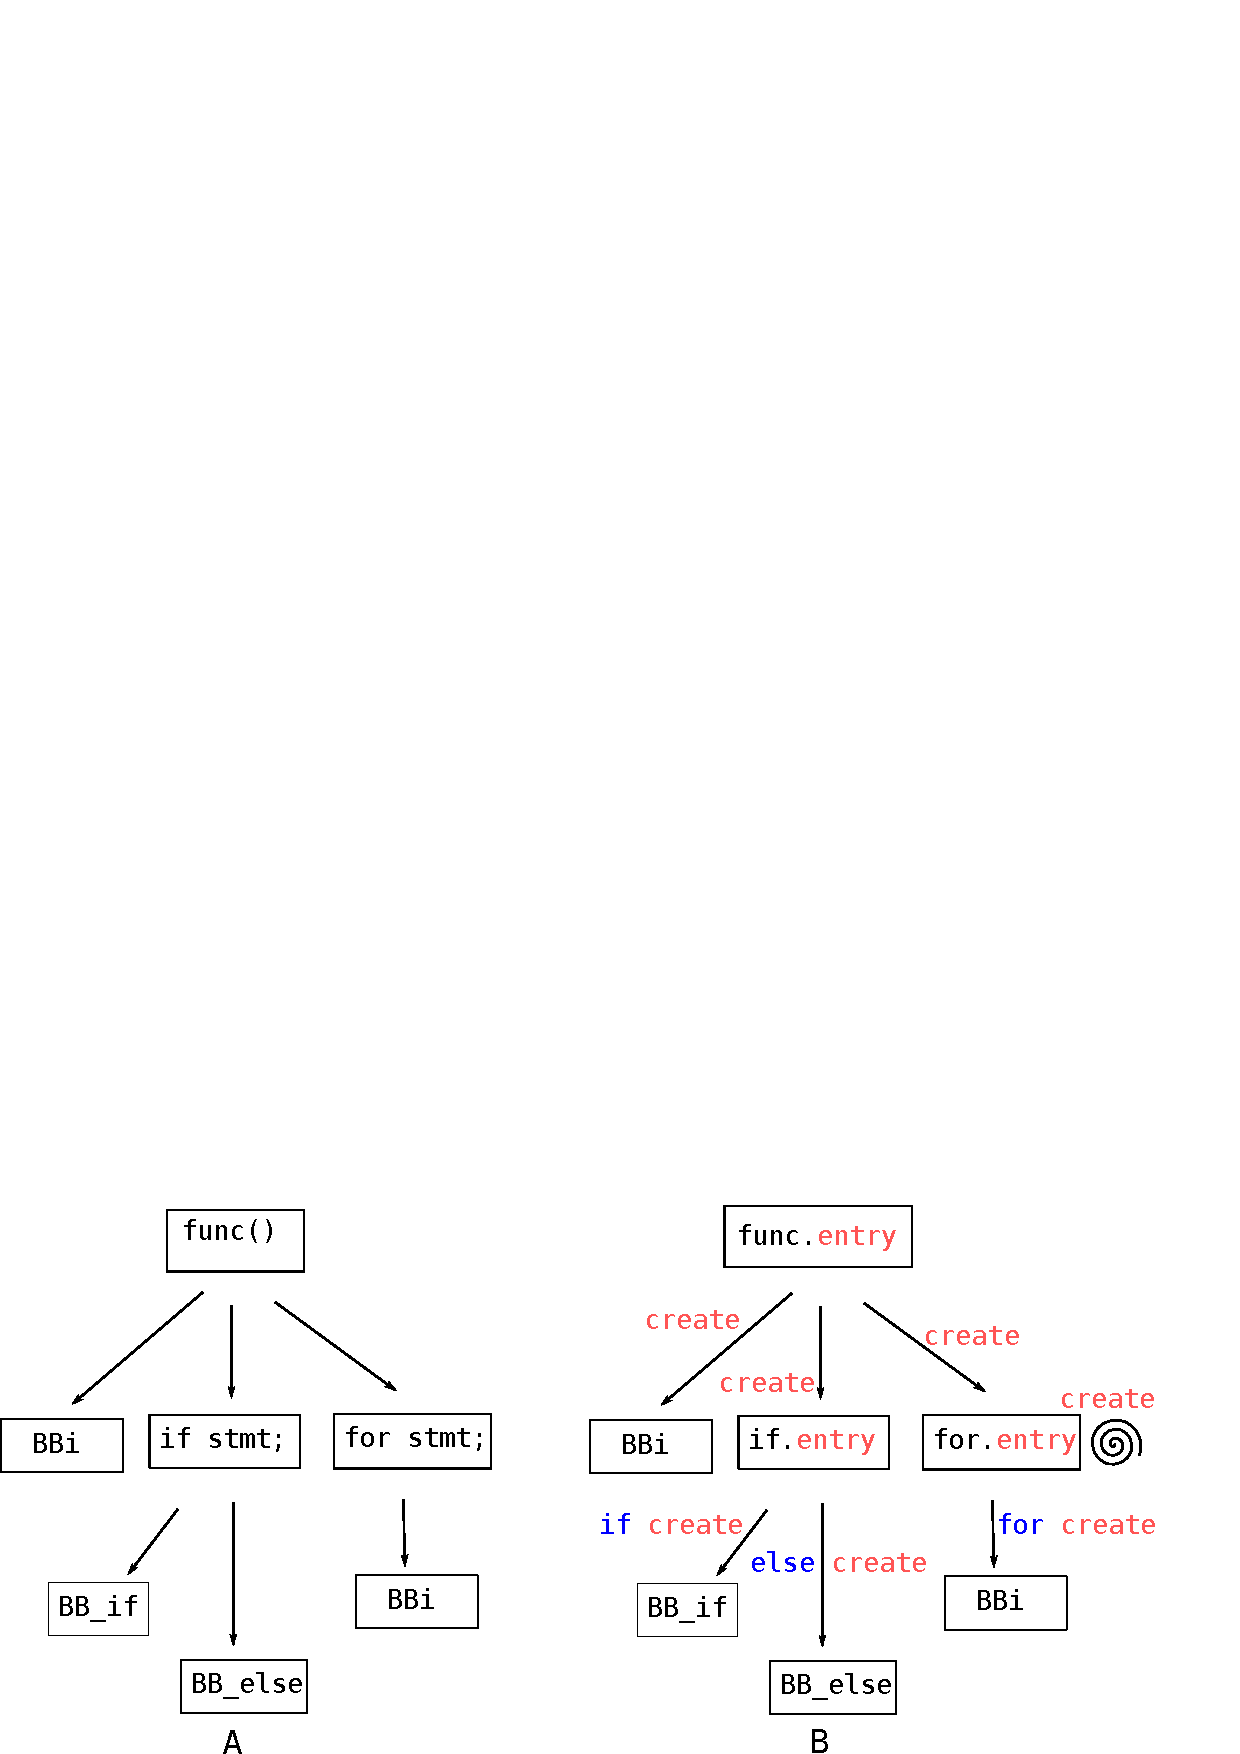
\includegraphics[width=.8\columnwidth]{jittc.pdf}

  \begin{itemize}
  \item Every non-leaf node in the \emph{control dependence graph}
    is a thread creation point
  \item Thread creation is conditional on the predicate at the
    source of the control dependence
  \item Input arguments and pointers to the frames of the dependent
    frame are collected from the def-use chains (see SSA form)
  \end{itemize}
\end{frame}

\begin{frame}[t]{General Conversion of control flow to data flow}
  Problem: in general, the consumer is not known at production time!

  \medskip
  \includegraphics[width=.6\columnwidth]{cdg4.pdf}

  \begin{itemize}
  \item When creating the thread for bb1, the frame pointer of its
    consumer is unknown, and it is not even sure there will be one
  \end{itemize}
\end{frame}

\begin{frame}[t]{General Conversion of control flow to data flow}
  Problem: in general, the consumer is not known at production time!

  \medskip
  \begin{minipage}{.40\textwidth}
    \includegraphics[width=.98\columnwidth]{cdg5.pdf}
  \end{minipage}
  \hfill
  \begin{minipage}{.50\textwidth}  
    \begin{itemize}
    \item When creating the thread for bb1, the frame pointer of its
      consumer is unknown, and it is not even sure there will be one
    \item Decompose the data dependence bb1$\to$bb4 into
      bb1$\to$bb2 and bb2$\to$bb4
    \item Additional dependence: frame pointer of bb2 passed through
      entry to bb1
    \end{itemize}
  \end{minipage}
\end{frame}

\begin{frame}{Caveats of Data-Driven Execution}
  \begin{block}{Performance}
    \begin{itemize}
    \item \color{gray}Dynamic memory management (heap object)
    \item \color{gray}Garbage collection
    \item \color{gray}Blindness of task scheduler w.r.t.\ future
      synchronizations
      \begin{itemize}
      \item \color{gray}The critical path is hidden
      \item \color{gray}Non-urgent future values waste precious local
        memory resources
      \end{itemize}
    \item \color{gray}Non-locality of future values w.r.t.\ their
      binding (consumer) tasks
    \item \color{gray}Memory consumption of suspended, waiting tasks
    \item \color{gray}Scheduling overhead of task suspension
    \end{itemize}
  \end{block}
  
  \begin{block}{Expressiveness}
    \begin{itemize}
    \item Strong restriction: the consumer always need to be known at
      thread (task) creation time
    \item This can be relaxed into letting a thread know about its
      consumers through specific input arguments, provided later than
      creation time but prior to thread (task) scheduling, at the cost
      of additional dependences for transverse data dependences
      (relative to the control dependence graph)
    \item Allows to implement futures, hence arbitrary dynamic
      dependences, but cumbersome: need for ``proxy'' threads, cloning
      themselves upon the binding of a future (\texttt{get()})
    \end{itemize}
  \end{block}
\end{frame}

\section{Synchronization  Structures}

\begin{frame}{Implementing Dependences Using Explicit Synchronizations}
  Arvind and Nikhil's I-structures

  Book: \textit{Implicit parallel programming in pH}, 2001.

  \hfill\includegraphics[width=3cm]{arvind}

  \bigskip
  I-structures: infinite, operational indexed streams, with
  \emph{full/empty} bits, Single-Producer-Multiple-Consumers (SPMC)

  \begin{itemize}
  \item I-structures where introduced for in-place operations in
    data-flow programs
  \item Kahn networks provide a functional definition (and
    denotational semantics)
  \item Does \emph{not} depend on a task scheduler to enforce dependences
  \item Caveats:
    \begin{itemize}
    \item No load balancing
    \item Cumbersome interaction with user-level thread scheduling:
      blocking a coroutine blocks the underlying worker (POSIX)
      thread, suspension needed
    \end{itemize}
  \end{itemize}

  Implementation: stream buffer, circular window (bounded), vector of futures
\end{frame}

\begin{frame}{Implementations of Concurrent Single-Assignment Streams}
  \begin{itemize}
  \item SPSC: only needs a store-store fence (free on x86-TSO)
  \item SPMC/MPSC: needs an atomic operation
  \item MPMC: often implemented using SPMC + MPSC (useful for data parallelism)

    \centerline{\includegraphics[width=7cm]{MPMC_consensus}}

    FastFlow is currently one of the best implementations:

    \url{http://mc-fastflow.sourceforge.net}

    \bigskip
  \item Indexed-based MPMC: only need a store-store fence!

    \centerline{\includegraphics[width=11cm]{MPMC_index-based}}

    \hfill\footnotesize In collaboration with Antoniu Pop and Cupertino Miranda
  \end{itemize}
\end{frame}

\begin{frame}{Fast Implementations of SPSC Streams}
  Circular buffer with two pointers/indexes

  \begin{itemize}
  \item Issue: detect full buffers with back-pressure

    \centerline{\includegraphics[width=11cm]{backpressure}}

  \item Simplest and most efficient solution for powers of two: absolute indexes
   
    Need arithmetic care to deal with wrap-arounds and (32bit) overflows
  \item Cache-aware optimization
    \begin{itemize}
    \item Manual/software caching of the last index
    \end{itemize}
  \end{itemize}
\end{frame}

\begin{frame}[t]{Fast Implementations of Index-Based MPMC Streams}
  \centerline{\scalebox{.6}{\input{intuition.pdf_t}}}

  \begin{block}{Stream synchronization primitives}
    \begin{itemize}
    \item \code{commit()}/\code{update()}: pressure
    \item \code{release()}/\code{stall()}: back-pressure
    \item \code{receive()}: prefetch on a sliding window
    \item Deterministic initialization protocol and
      garbage collection of dead sliding windows
    \end{itemize}
  \end{block}

  \begin{block}{Lightweight runtime}
    Circular buffer with two sets of indexes, for the producer and
    consumer sides

    \begin{itemize}
    \item Cache the minimum of the producer (resp.\ consumer) indexes
    \item Cache-aware optimization
      \begin{itemize}
      \item Manual/software caching of the last index
      \item Monotonicity tolerates race-conditions on minimum index computation
      \item Alignment of shared indexes on a cache line alignment to
        avoid false sharing
      \end{itemize}
    \end{itemize}
  \end{block}
\end{frame}

\begin{frame}[t]{Fast Implementations of Index-Based MPMC Streams}
  \centerline{\scalebox{.6}{\input{intuition.pdf_t}}}

  \bigskip
  \centerline{\includegraphics[width=5cm]{cache_optimized_update}}
\end{frame}

\begin{frame}[t]{Fast Implementations of Index-Based MPMC Streams}
  \centerline{\scalebox{.6}{\input{intuition.pdf_t}}}

  \bigskip
  \centerline{\includegraphics[width=8cm]{erbium_fences}}
\end{frame}

\begin{frame}[t]{Fast Implementations of Index-Based MPMC Streams}
  \centerline{\scalebox{.6}{\input{intuition.pdf_t}}}

  \begin{block}{Lightweight runtime}
    \begin{itemize}
    \item Lock-free, consensus-free implementation
      \begin{itemize}
      \item No hardware atomic instruction
      \item No memory fence with x86-TSO memory model
      \end{itemize}
    \item $\approx10$ cycles per streaming communication cycle
    \item Compatible with a work-stealing scheduler
    \end{itemize}
  \end{block}
\end{frame}

\begin{frame}[fragile]{Evaluation on a Synthetic Benchmark}
  \begin{center}
    \includegraphics[width=.8\columnwidth]{exploration_cilk}

    \medskip
    Core 2 Duo -- 4 cores
  \end{center}
\end{frame}

\begin{frame}[fragile]{Evaluation on FFT}
  \begin{center}
    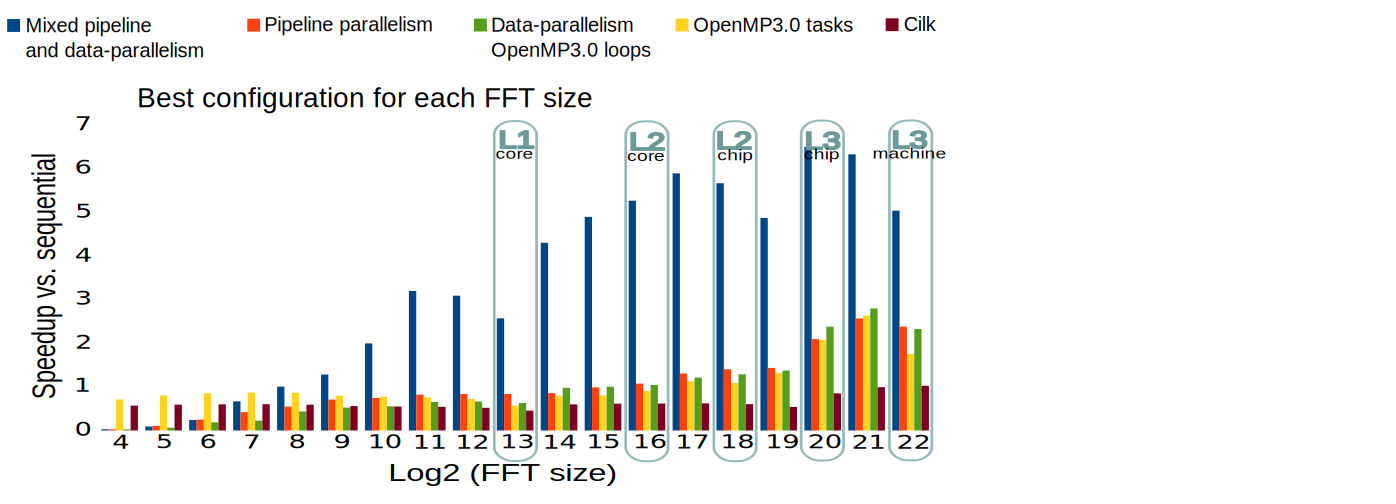
\includegraphics[width=1.4\columnwidth]{fft_opteron.pdf}

    \medskip
    4-socket~Opteron~--~16~cores
  \end{center}
\end{frame}

\section{Message}

\begin{frame}{Message}
  \begin{alertblock}{}
    Control-flow: tasks and futures

    Data-flow: data-driven threads (tasks)

    Synchronization structures: threads and streams

    \medskip
    \centerline{$\to$ all have pros and cons... working on a unifying principle}
  \end{alertblock}
  
  \begin{alertblock}{}
    \Large\color{darkgreen}
    Hope: parallel programming can be both safe and efficient!
  \end{alertblock}

  \bigskip
  Acknowledgments:
  
  \medskip
  \qquad\begin{minipage}{5cm}
    Léonard Gérard
    
    Feng Li
    
    Cupertino Miranda
    
    Antoniu Pop
  \end{minipage}
\end{frame}

% \begin{frame}{Next Courses}
%   \begin{itemize}
%   \item Wrap-up on kernel and programming language memory
%     models by Francesco

%     \bigskip
%   \item Parallel language and compilers for deterministic multicore programming

%     \bigskip
%   \item Concurrent data-structures by Luc
%   \end{itemize}
% \end{frame}

\end{document}
